\section{Initial Value Problems}\label{sec11}
\textit{Initial value problems} are nothing but differential equations that require finding solutions, given the initial conditions at time $t_0$.
\begin{equation}\label{eq101}
\dot{y} = f(t, y) \; with \; y_0 = y(t_0)
\end{equation}
The problem as described in \cref{eq101} is an \textit{ordinary differential equation} of the first order. One can determine the solution analytically using \cref{eq102}.
\begin{equation}\label{eq102}
y(t) = y_0 + \int_{t_0}^{t} f(\tau, y(\tau)) \, d\tau
\end{equation}
In this case, the integral in \cref{eq102} needs to be determined in order to find the solution for time interval of interest. Though it may seem easy, it is often a herculean task to evaluate this integral, particularly when $f(\tau, y(\tau))$ is a non-linear function. 

Furthermore, initial value problems with \textit{higher order} differential equations can be transformed into a system of differential equations and expressed in a vectorized form as shown below.
\begin{equation}\label{eq103}
\begin{gathered}
\dot{\mathit{Y}} = F (t,\mathbf{A}, \mathit{Y}, B) \; with \; \mathit{Y_0} = \mathit{Y}(t_0) \\
\\
\text{where, } 
\mathit{Y} = \begin{pmatrix}
           y_{1}(t) \\
           y_{2}(t) \\
           \vdots \\
           y_{n}(t)
         \end{pmatrix}
\text{, } 
\mathit{\dot{Y}} = \begin{pmatrix}
           \dot{y}_{1}(t) \\
           \dot{y}_{2}(t) \\
           \vdots \\
           \dot{y}_{n}(t)
         \end{pmatrix}
\text{, }
\mathit{Y_0} = \begin{pmatrix}
           y_{1}(t_0) \\
           y_{2}(t_0) \\
           \vdots \\
           y_{n}(t_0)
         \end{pmatrix}
\end{gathered}
\end{equation}

A solution to the formulations as described in \cref{eq103}, where $
\mathbf{A}$ is the System Matrix and $B$ is the Excitation Vector, using a procedure like in \cref{eq102} is complicated often not possible. Hence, it is sought to approximate them numerically using methods that will be discussed hereafter.

\section{Numerical Time Integration Schemes}
\label{sec:timeintegration}
\subsection{Explicit Euler Method}
The Explicit Euler time integration scheme was the first method developed to solve initial value problems. In this scheme, the time derivative $\dot{y}(t)$ in \cref{eq101} is calculated using the \textit{forward difference method}. Therefore, as we march forward in time, the new values of the solution are computed using only known values of the solution at the previous time step \parencite[see][pg. 97]{Fuhrer2001}. 

In short, the Explicit Euler time integration scheme can be summarized as
\begin{equation}
\label{eq104}
y_{n+1} = y_n + h f(t_n, y_n) \text{\hspace{15mm}} n = 0,1,\ldots\\ \\
\end{equation}
where, $y_0 = y(t_0)$ is the initial condition and $h = t_{n+1} - t_n$ is the time increment interval.

The algorithm for procedural implementation of the Explicit Euler time integration scheme is as shown below:
\begin{center}
\smallskip
\begin{minipage}{.7\linewidth}
    \begin{algorithm}[H]
      \SetAlgoLined
      \KwData{$h, n, f(t, y), y_0, t_0$}
      \KwResult{$y_{exp}=\{y_0, y_1, \ldots, y_n\}$ 
      			at $t=\{t_0, t_1, \ldots, t_n\}$ }
      Initialize arrays $y_{exp}=\{y_0\}$ and $t=\{t_0\}$\;
      $y_{i} \gets y_0$ and $t_{i} \gets t_0$\;
      \For{$i \gets 0$ \textbf{to} $n$}  { 
      $y_{i+1} = y_{i} + h f(t_i, y_i)$\;
      $t_{i+1} = t_{i} + h$\;
      Append $y_{exp} \gets y_{i+1}$;
      Append $t \gets t_{i+1}$;
      }
      \Return{$y_{exp}, t$}
     \caption{Explicit Euler Time Integration}
	\label{algo:exp_euler}
    \end{algorithm}
  \end{minipage}
\end{center}

Although this method is fast and can implemented numerically with ease, it is only \textit{conditionally stable} \cite[see][]{Fuhrer2001}. An implementation of the Explicit Euler time integration scheme in python can be found in Appendix A.

\subsection{Implicit Euler Method}\label{sec:implicitEuler}
The Implicit Euler time integration scheme is used to alleviate the stability issues of the Explicit Euler Method. In this scheme, the time derivative $\dot{y}(t)$ in \cref{eq101} is calculated using the \textit{backward difference method}. Therefore, as we march forward in time, the new values of the solution cannot be computed explicitly using known values of the solution at the previous time step \parencite[see][pg. 105]{Fuhrer2001}.
\begin{equation}
\label{eq105}
y_{n+1} = y_n + h f(t_{n+1}, y_{n+1}) \text{\hspace{15mm}} n = 0,1,\ldots\\ 
\end{equation}
where, $y_0 = y(t_0)$ is the initial condition and $h = t_{n+1} - t_n$ is the time increment interval.

It is evident from \cref{eq105} that calculating the solution at the next time step is not straigt forward. However, using the a few mathematical tools that are explined further, the Implicit Euler time integration scheme can be numerically solved.

\subsubsection{Analytical Reformulation}
Given \cref{eq101}, the derivative of the function at every time step can be calculated. Thus, for the time $t_{n+1}$ the we have
\begin{equation}
\dot{y}_{n+1} = f(t_{n+1}, y_{n+1})
\label{eq106}
\end{equation}

Furthermore, \cref{eq105} can be rewritten as 
\begin{equation}
\label{eq107}
y_{n+1} = y_n + h {\dot{y}_{n+1}}
\end{equation}
Now by combining \cref{eq106} and \cref{eq107}, the Implicit Euler time integration scheme can be formulated using only the values of solution ${y_n}$ at previous time step. \parencite[see][]{andasarihandout}
\begin{equation}
\label{eq108}
y_{n+1} = y_n + f(h, t_{n+1}, y_{n}) \\
\end{equation}

As an example of this method, the Implicit Euler time integration scheme for \cref{eq109} can be formulated as shown in \cref{eq110} below.
\begin{equation}
\label{eq109}
\dot{y} = \lambda (y - \sin(t)) + \cos(t)
\end{equation}
\begin{equation}
\label{eq110}
\begin{gathered}
y_{n+1} = y_n + \dfrac{h}{1-h\lambda}f(t_{n+1}, y_{n}) \\
\text{for } n = 0,1,\ldots\\ 
\end{gathered}
\end{equation}

Using the formulation in \cref{eq108}, numerical implementation with time marching is now straightforward. The algorithm for this implementation is as follows:
\begin{center}
\smallskip
\begin{minipage}{.7\linewidth}
    \begin{algorithm}[H]
      \SetAlgoLined
      \KwData{$h, n, f(h, t, y), y_0, t_0$}
      \KwResult{$y_{imp}=\{y_0, y_1, \ldots, y_n\}$ 
      			at $t=\{t_0, t_1, \ldots, t_n\}$ }
      Initialize arrays $y_{imp}=\{y_0\}$ and $t=\{t_0\}$\;
      $y_{i} \gets y_0$ and $t_{i} \gets t_0$\;
      \For{$i \gets 0$ \textbf{to} $n$}  { 
	  $t_{i+1} = t_{i} + h$\;      
      $y_{i+1} = y_{i} + f(h, t_{i+1}, y_i)$\;
      Append $y_{exp} \gets y_{i+1}$;
      Append $t \gets t_{i+1}$;
      }
      \Return{$y_{imp}, t$}
     \caption{Implicit Euler Time Integration - \\%
     using Analytical Reformulation}
	\label{algo:imp_euler_analytical}
    \end{algorithm}
  \end{minipage}
\end{center}

In addition to an easy numerical implementation, this scheme is also \textit{uncondtionally stable}. However, the function $f(h, t, y)$ needs to be found out manually for each problem, thus, limiting its applicability to simple problems and predominantly scalar valued functions $f(t, y)$. 

\subsubsection{Matrix Inversion}
Using \cref{eq109} as an example, \cref{eq107} can be evaluated for $n = 0, 1, 2\ldots$ as
\begin{align}
\label{eq111}
\begin{aligned}
y_{1} &= y_0 + h [\lambda (y_1 - \sin(t_1)) + \cos(t_1)]\\
y_{2} &= y_1 + h [\lambda (y_2 - \sin(t_2)) + \cos(t_2)]\\
\vdots\\
y_{n} &= y_{n-1} + h [\lambda (y_n - \sin(t_n)) + \cos(t_n)]
\end{aligned}
\end{align}
The linear set of equations in \cref{eq111} can be rearranged into \cref{eq112} and then written in matrix form as shown in \cref{eq113}. After inverting the matrix $\mathbf{A}$, we can solve for $\mathbf{y}$ using \cref{eq114}
\begin{align}
\label{eq112}
\begin{aligned}
(1 - h\lambda)y_{1} &= h [\lambda (-\sin(t_1)) + \cos(t_1)] + y_0 \\
(1 - h\lambda)y_{2} - y_1 &= h [\lambda (-\sin(t_2)) + \cos(t_2)]\\ 
\vdots\\
(1 - h\lambda)y_{n} - y_{n-1} &= h [\lambda (-\sin(t_n)) + \cos(t_n)]\\
\end{aligned}
\end{align}
\begin{gather}\label{eq113}
\begin{gathered}[t]
\mathbf{A} \mathbf{y} = \mathbf{b}\\ \\ 
\text{where, } \mathbf{A} = 
\begin{bmatrix}
           (1 - h\lambda) & 0 & \ldots & 0 & 0\\
           -1 & (1 - h\lambda) & \ldots & 0 & 0\\
           \vdots & \vdots & \ddots & \vdots & \vdots\\
           0 & 0 & \ldots & (1 - h\lambda) & 0\\
           0 & 0 & \ldots & -1 & (1 - h\lambda)
\end{bmatrix} \\ \\
\mathbf{y} =
\begin{pmatrix}
           y_{1}\\
           y_{2}\\
           \vdots \\
           y_{n-1}\\
           y_{n}
\end{pmatrix} \text{ and } 
\mathbf{b}=
\begin{pmatrix}
           h [\lambda (-\sin(t_1)) + \cos(t_1)] + y_0\\
           h [\lambda (-\sin(t_2)) + \cos(t_2)]\\
           \vdots \\
           h [\lambda (-\sin(t_{n-1})) + \cos(t_{n-1})]\\
           h [\lambda (-\sin(t_n)) + \cos(t_n)]
\end{pmatrix} 
\end{gathered}
\end{gather}
\begin{equation}
\label{eq114}
\mathbf{y} = \mathbf{A^{-1}} \mathbf{b}
\end{equation}

An algorithm for this implementation is as follows:
\begin{center}
\smallskip
\begin{minipage}{.7\linewidth}
    \begin{algorithm}[H]
      \SetAlgoLined
      \KwData{$h, n, y_0, t_0$}
      \KwResult{$y_{imp}=\{y_0, y_1, \ldots, y_n\}$ 
      			at $t=\{t_0, t_1, \ldots, t_n\}$ }
      Initialize arrays $y_{imp}=\{y_0\}$ and $t=\{t_0\}$\;
	  Initialize vector $\mathbf{b}$ and matrix $\mathbf{A}$\;    
      Setup vector $\mathbf{b}$\; \tcp*[f]{Append $t \gets t_i$ for every row}\; 
      Setup matrix $\mathbf{A}$\;
      Calculate $\mathbf{A^{-1}}$\;
      Calculate $\mathbf{y_{sol}} \gets \mathbf{A^{-1}} \mathbf{b}$\;
      Append $y_{imp} \gets \mathbf{y_{sol}}$\;
      \Return{$y_{imp}, t$}
     \caption{Implicit Euler Time Integration - \\
     using Matrix Inversion}
	\label{algo:imp_euler_matrix}
    \end{algorithm}
  \end{minipage}
\end{center}

Although $\mathbf{A}$ is a sparse matrix, the availability of sophisticated matrix inversion methods for sparse matrices makes the solution of this formulation easily possible. An additional benefit is the elimination of forward time marching. Thus, the solution for the entire time domain is calculated at once. It is, however, important to note that when dealing with initial value problems of higher-order, the size of $\mathbf{A}$ would increase quickly and could lead to problems during matrix inversion. 

\subsubsection{Fixed Point Iteration}\label{sec:implicitEulerIterative}
A fixed point iteration can be applied to solve \cref{eq105}. \parencite[See][pg. 105]{Fuhrer2001}. Thus, we have the following reformulation for the Implicit Euler time integration scheme 
\begin{gather}
\label{eq115}
\begin{gathered}
y^{(j+1)}_{n+1} = y_n + h f(t_{n+1}, y^{(j)}_{n+1}) \\
\text{\hspace{15mm}} j = 0,1,\ldots
\end{gathered}
\end{gather}
In this way, for every step forward in time, we perform additional iterations to converge to a solution. In order to find an initial guess $y^{(0)}_{n+1}$, the Explicit Euler scheme can be used as given in \cref{eq116}. This formulation, thus, comes under the the class of Predictor-Corrector schemes for solving initial value problems.
\begin{equation}
\label{eq116}
y^{(0)}_{n+1} = y_n + h f(t_n, y_n)
\end{equation}
The algorithm for procedural implementation of the Implicit Euler time integration scheme with Fixed Point Iteration is as shown below:
\begin{center}
\smallskip
\begin{minipage}{.7\linewidth}
    \begin{algorithm}[H]
      \SetAlgoLined
      \KwData{$h, n, f(t, y), y_0, t_0, iter_{max}$}
      \KwResult{$y_{imp}=\{y_0, y_1, \ldots, y_n\}$ 
      			at $t=\{t_0, t_1, \ldots, t_n\}$ }
      Initialize arrays $y_{imp}=\{y_0\}$ and $t=\{t_0\}$\;
      Set $convergence \gets True$\; 
      $y_{i} \gets y_0$ and $t_{i} \gets t_0$\;
      \For{$i \gets 0$ \textbf{to} $n$}  {
      	\If{$convergence$} {
		  Initialize $err \gets 1$ and $j \gets 0$\;		  	
		  $y^{j}_{i+1} = y_{i} + h f(t_{i}, y_{i})$\;		  	
		  $t_{i+1} = t_{i} + h$\;
		  \While{$convergence$} {
			$y^{j+1}_{i+1} = y_{i} + h f(t_{i+1}, y^{j}_{i+1})$\;
			$err = abs(y^{j+1}_{i+1} - y^{j}_{i+1})$\;
			$j \gets j+1$\;
			\If(\tcp*[f]{Solution Converged}){$err < tol$}{ 
			  $y_{i+1} = y^{j+1}_{i+1}$\;
    	 	  Append $y_{imp} \gets y_{i+1}$\;
      		  Append $t \gets t_{i+1}$\;
      		  \textbf{break}\;
      		}
      		\If(\tcp*[f]{Solution Diverged}){$j > iter_{max}$}{ 
			  $convergence \gets False$
      		}
      	  }
      	}
      }
      \Return{$y_{imp}, t$}
     \caption{Implicit Euler Time Integration - using Fixed Point Iteration}
	\label{algo:imp_euler_analytical}
    \end{algorithm}
  \end{minipage}
\end{center}
It is important to note that, although this is an Implicit Euler time integration scheme, using fixed point iteration renders this scheme to be \textit{conditionally stable}.

Again, python code implementations for all the Implicit Euler time integration schemes discussed above can be found in Appendix A. 


\subsection{Comparison of Euler Time Integration Schemes}
\begin{figure}[h]
\begin{subfigure}{0.5\textwidth}
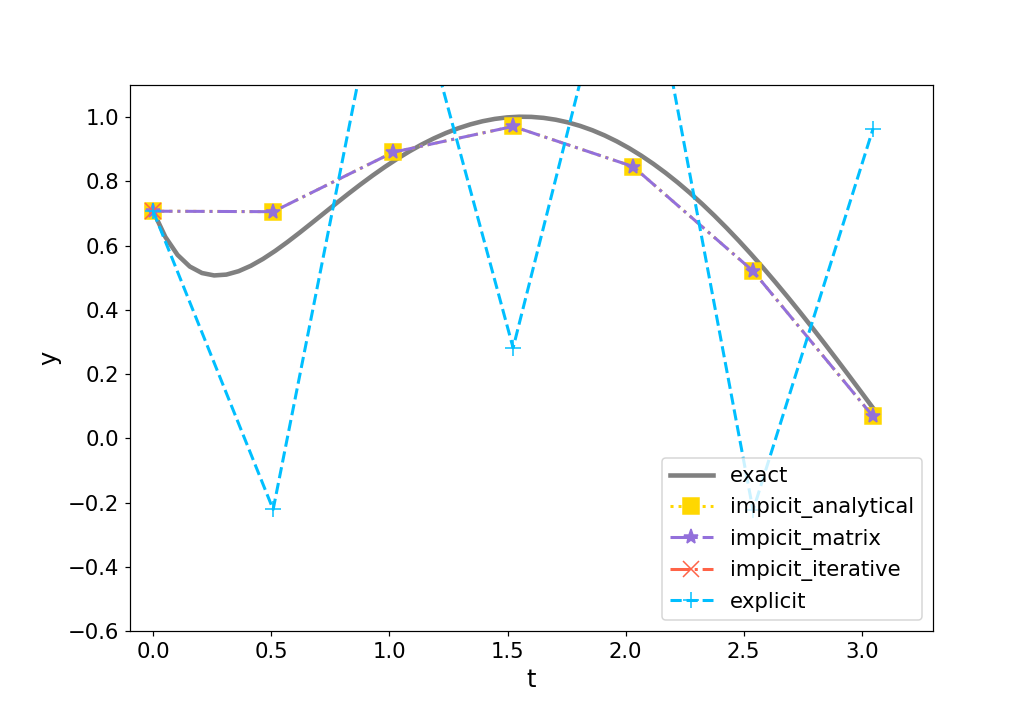
\includegraphics[width=\linewidth]{eulercomp1} 
\caption{$\lambda = -4.0, h = 0.5$}
\label{fig:eulercomp1}
\end{subfigure}
\begin{subfigure}{0.5\textwidth}
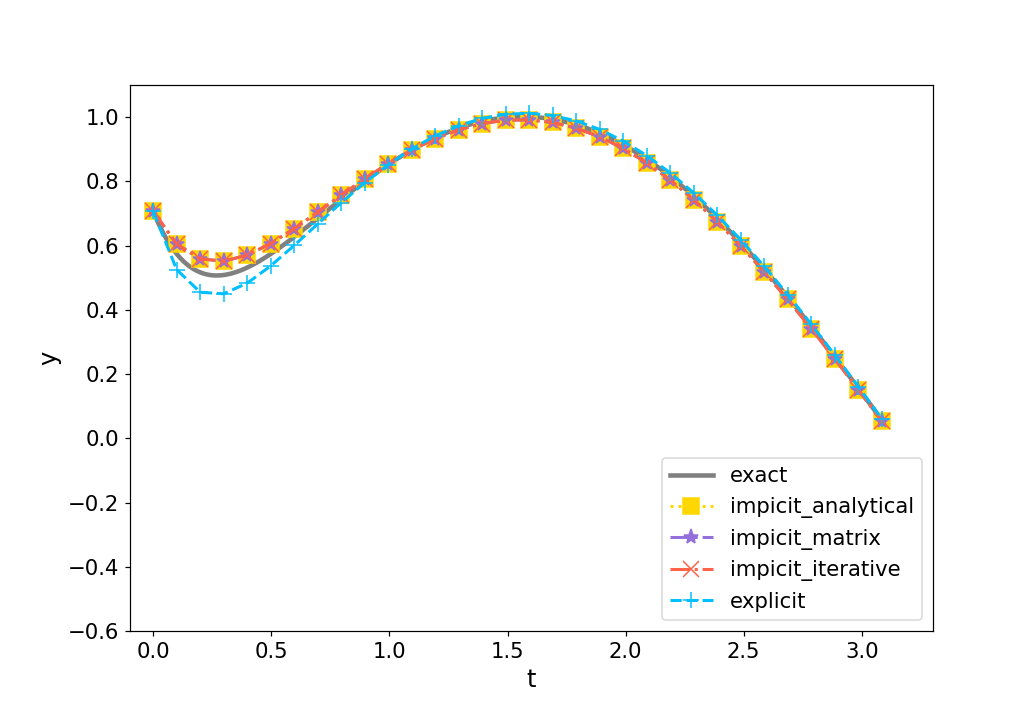
\includegraphics[width=\linewidth]{eulercomp2}
\caption{$\lambda = -4.0, h = 0.1$}
\label{fig:eulercomp2}
\end{subfigure}
\begin{subfigure}{0.5\textwidth}
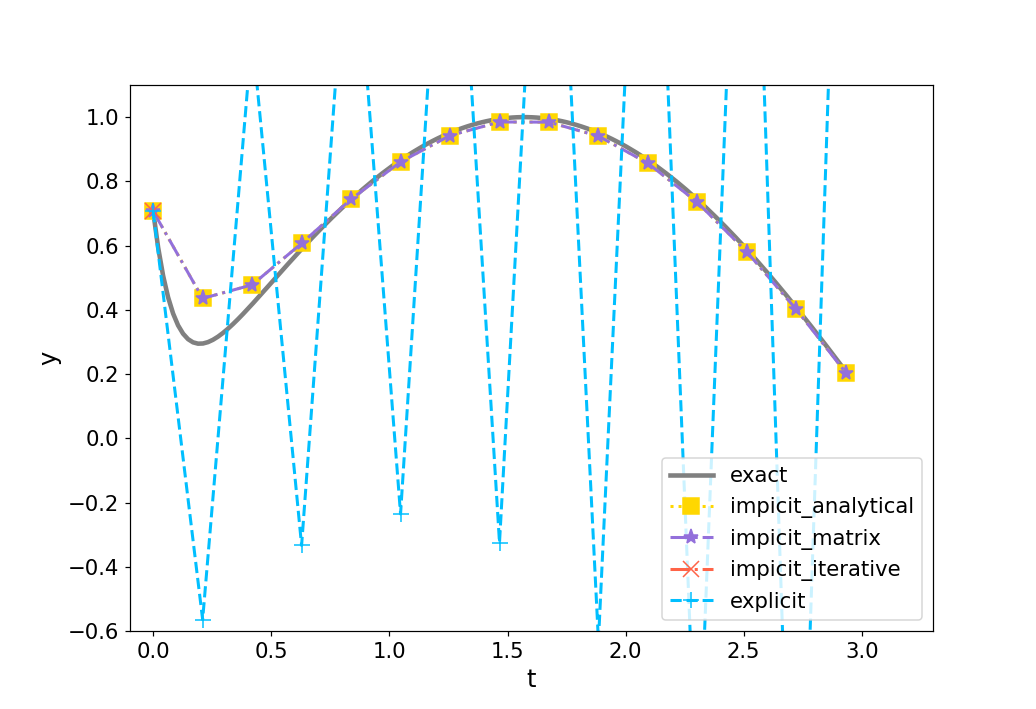
\includegraphics[width=\linewidth]{eulercomp3} 
\caption{$\lambda = -10.0, h = 0.2$}
\label{fig:eulercomp3}
\end{subfigure}
\begin{subfigure}{0.5\textwidth}
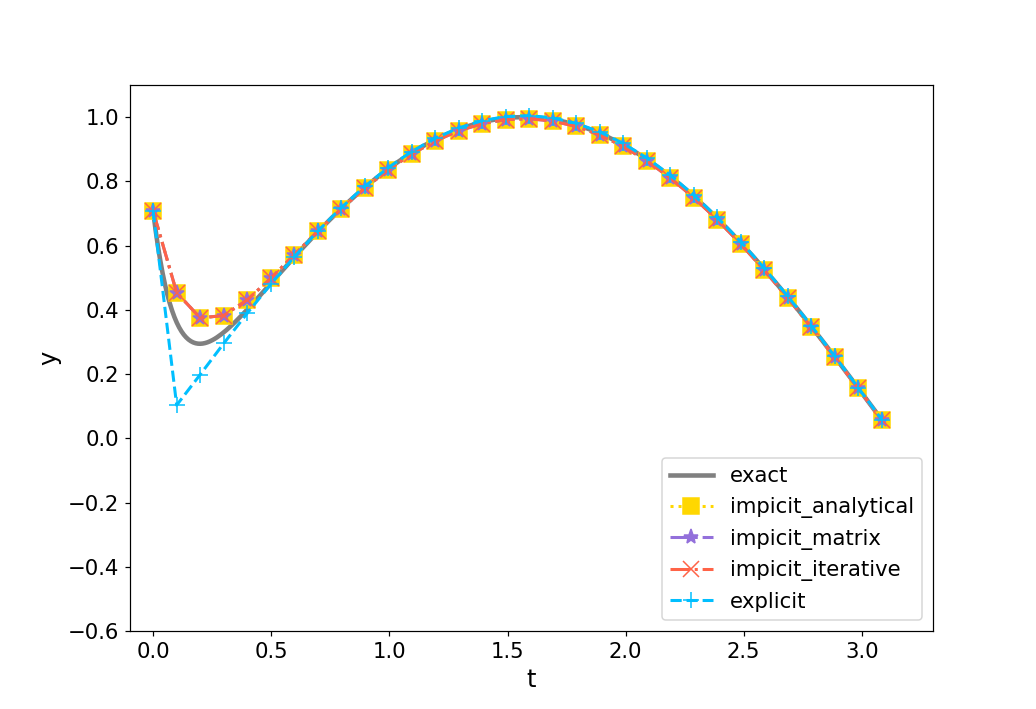
\includegraphics[width=\linewidth]{eulercomp4}
\caption{$\lambda = -10.0, h = 0.1$}
\label{fig:eulercomp4}
\end{subfigure}
\begin{subfigure}{\textwidth}
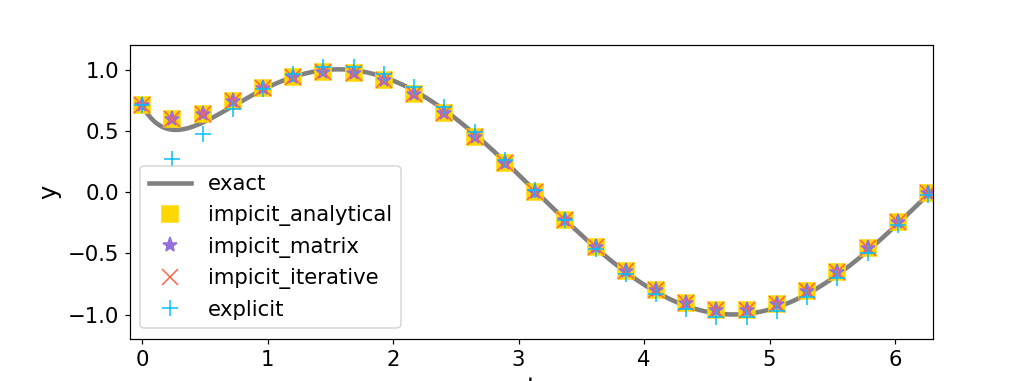
\includegraphics[width=\linewidth]{eulercomp5} 
\caption{$\lambda = -4, h = 0.24$}
\label{fig:eulercomp5}
\end{subfigure}
\caption{Solution to $\dot{y} = \lambda (y - \sin(t)) + \cos(t),\; y(0) = 1/\sqrt{2}$}
\label{fig:eulerComparison}
\end{figure}
A graphical representation showing solutions to \cref{eq109} with initial condition $y(0) = 1/\sqrt{2}$, solved with all the above stated time integration schemes with varying parameters $\lambda$ and $h$ can be found in \cref{fig:eulerComparison}. It can be observed that all the three Implicit Euler time integration schemes lead to the same solution. The analytical solution for this initial value problem is given below
\begin{equation}
\label{eq117}
y = (y_0 - \sin t_0)\exp^{\lambda(t-t_0)} + \sin t
\end{equation}


\section{Solution to Example Problems}

// TODO

Solution for $\dot{u} + \gamma u = f$

//TODO

Solution for $\beta \ddot{u} + \alpha \dot{u} + \lambda {u} = f$ - (Only graphs)
Detailed solution will be discussed in next chapter due to similarity with equation of motion
